% Copyright 2006 by Till Tantau
%
% This file may be distributed and/or modified
%
% 1. under the LaTeX Project Public License and/or
% 2. under the GNU Free Documentation License.
%
% See the file doc/generic/pgf/licenses/LICENSE for more details.


\section{Guidelines on Graphics}

The present section is not about \pgfname\ or \tikzname, but about
general guidelines and principles concerning the creation of
graphics for scientific presentations, papers, and books.

The guidelines in this section come from different sources. Many of
them are just what I would like to claim is ``common sense,'' some
reflect my personal experience (though, hopefully, not my personal
preferences), some come from books (the bibliography is still missing,
sorry) on graphic design and typography. 
The most influential source  are the brilliant books
by Edward Tufte. While I do not agree with everything written in these
books, many of Tufte's arguments are so convincing that I decided to
repeat them in the following guidelines. 

The first thing you should ask yourself when someone presents a bunch of
guidelines is: Should I really follow these guidelines? This is an
important questions, because there are good reasons not to follow
general guidelines.  The person who setup the guidelines may have had other
objectives than you do. For example, a guideline might say ``use the
color red for emphasis.'' While this guideline makes perfect sense
for, say, a presentation using a projector, red ``color'' has the
\emph{opposite} effect of ``emphasis'' when printed using a
black-and-white printer. Guidelines were almost always setup to
address a specific situation. If you are not in this situation,
following a guideline can do more harm than good.

The second thing you should be aware of is the basic rule of
typography is: ``Every rule can be broken, as long as you are
\emph{aware}  that you are breaking a rule.'' This rule also applies
to graphics. Phrased differently, the basic rule states: ``The only
mistakes in typography are things done is ignorance.''  When you are
aware of a rule and when you decide that breaking the rule has a
desirable effect, break the rule.


\subsection{Planning the Time Needed for the Creation of Graphics}

When you create a paper with numerous graphics, the time needed to
create these graphics becomes an important factor. How much time
should you calculate for the creation of graphics?

As a general rule, assume that a graphic will need as much time to
create as would a text of the same length. For example, when I
write a paper, I need about one hour per page for
the first draft. Later, I need between two and four hours per page
for revisions. Thus, I expect to need about half an hour for the
creation of \emph{a first draft} of a half page graphic. Later on, I
expect another one to two hours before the final graphic is finished.

In many publications, even in good journals, the authors and editors
have obviously  invested a lot of time on the text, but seem to 
have spend about five minutes to create all of the
graphics. Graphics often seem to have been added as an
``afterthought'' or look like a screen shot of whatever the authors's
statistical software shows them. As will be argued later on, the
graphics that programs like \textsc{gnuplot} produce by default are of
poor quality.

Creating informative graphics that help the reader and that fit
together with the main text is a difficult, lengthy process. 
\begin{itemize}
\item
  Treat graphics as first-class citizens of your papers. They deserve
  as much time and energy as the text does.
  Indeed, the creation of graphics might deserve \emph{even more} time
  than the writing of the main text since more attention will  be paid
  to the graphics and they will be looked at first. 
\item
  Plan as much time for the creation and revision of a graphic as you
  would plan for text of the same size.
\item
  Difficult graphics with a high information density may require even
  more time.
\item
  Very simple graphics will require less time, but most likely you do
  not want to have ``very simple graphics'' in your paper, anyway;
  just as you would not like to have a ``very simple text'' of the
  same size.  
\end{itemize}


\subsection{Workflow for Creating a Graphic}

When you write a (scientific) paper, you will most likely follow the
following pattern: You have some results/ideas that you would
like to report about. The creation of the paper will typically start
with compiling a rough outline. Then, the different sections are
filled with text to create a first draft. This draft is then revised
repeatedly until, often after substantial revision, a final paper
results. In a good journal paper there is typically not be a single 
sentence that has survived unmodified from the first draft.

Creating a graphics follows the same pattern:
\begin{itemize}
\item
  Decide on what the graphic should communicate. Make this a conscious
  decision, that is, determine ``What is the graphic supposed to tell
  the reader?''
\item
  Create an ``outline,'' that is, the rough overall ``shape'' of the
  graphic, containing the most crucial elements. Often, it is
  useful to do this using pencil and paper.
\item
  Fill out the finer details of the graphic to create a first
  draft.
\item
  Revise the graphic repeatedly along with the rest of the paper.
\end{itemize}




\subsection{Linking Graphics With the Main Text}

Graphics can be placed at different places in a text. Either, they can
be inlined, meaning they are somewhere ``in the middle of the text''
or they can be placed in standalone ``figures.'' Since printers (the
people) like to have their pages ``filled,'' (both for aesthetic and
economic reasons) standalone figures may traditionally be placed on
pages in the document far removed from the main text that refers to
them. \LaTeX\ and \TeX\ tend to encourage this ``drifting away'' of
graphics for technical reasons. 

When a graphic is inlined, it will more or less automatically be
linked with the main text in the sense that the labels of the graphic
will be implicitly explained by the surrounding text. Also, the main
text will typically make it clear what the graphic is about and what
is shown.

Quite differently, a standalone figure will often be viewed at a time
when the main text that this graphic belongs to either has not yet
been read or has been read some time ago. For this reason, you should
follow the following guidelines when creating standalone figures:
\begin{itemize}
\item
  Standalone figures should have a caption than should make them
  ``understandable by themselves.''

  For example, suppose a graphic shows an example of the different
  stages of a quicksort algorithm. Then the figure's caption should,
  at the very least, inform the reader that ``The figure shows the
  different stages of the quicksort algorithm introduced on page
  xyz.'' and not just ``Quicksort algorithm.''
\item
  A good caption adds as much context information as possible. For
  example, you could say: ``The figure shows the different stages of
  the quicksort algorithm introduced on page xyz. In the first line,
  the pivot element 5 is chosen. This causes\dots'' While this
  information can also be given in the main text, putting it in the
  caption will ensure that the context is kept. Do not feel afraid of
  a 5-line caption. (Your editor may hate you for this. Consider
  hating them back.)
\item
  Reference the graphic in your main text as in ``For an example of
  quicksort `in action,' see Figure~2.1 on page xyz.''
\item
  Most books on style and typography recommend that you do not use
  abbreviations as in ``Fig.~2.1'' but write ``Figure 2.1.''

  The main argument against abbreviations is that ``a period is too
  valuable to waste it on an abbreviation.'' The idea is that a period
  will make the reader assume that the sentence ends after ``Fig'' and
  it takes a ``conscious backtracking'' to realize that the sentence
  did not end after all.

  The argument in favor of abbreviations is that they save space.
  
  Personally, I am not really convinced by either argument. On the one
  hand, I have not yet seen any hard evidence that abbreviations slow 
  readers down. On the other hand,  abbreviating all ``Figure'' by
  ``Fig.''\ is most unlikely to save even a single line in  most
  documents. I avoid abbreviations.
\end{itemize}



\subsection{Consistency Between Graphics and Text}

Perhaps the most common ``mistake'' people do when creating graphics
(remember that a ``mistake'' in design is always just ``ignorance'')
is to have a mismatch between the way their graphics look and the way 
their text looks.

It is quite common that authors use several different programs for
creating the graphics of a paper. An author might produce some plots
using \textsc{gnuplot}, a diagram using \textsc{xfig}, and include an
|.eps| graphic a coauthor contributed using some unknown program. All
these graphics will, most likely, use different line widths, different
fonts, and have different sizes. In addition, authors often use
options like |[height=5cm]| when including graphics to scale them to
some ``nice size.''

If the same approach were taken to writing the main text, every
section would be written in a different font at a different size. In
some sections all theorems would be underlined, in another they would
be printed all in uppercase letters, and in another in red. In
addition, the margins would be different on each page.
Readers and editors would not tolerate a text if it were written in
this fashion, but with graphics they often have to.

To create consistency between graphics and text, stick to the
following guidelines:
\begin{itemize}
\item
  Do not scale graphics.

  This means that when generating graphics using an external program,
  create them ``at the right size.''
\item
  Use the same font(s) both in graphics and the body text.
\item
  Use the same line width in text and graphics.

  The  ``line width'' for normal text is the width of the stem of
  letters like T{}. For \TeX, this is usually
  $0.4\,\mathrm{pt}$. However, some journals will not accept graphics
  with a normal line width below $0.5\,\mathrm{pt}$.
\item
  When using colors, use a consistent color coding in the text and in  
  graphics. For example, if red is supposed to alert the reader to
  something in the main text, use red also in graphics for important
  parts of the graphic. If blue is used for structural elements like 
  headlines and section titles, use blue also for structural elements
  of your graphic.

  However, graphics may also use a logical intrinsic color
  coding. For example, no matter what colors you normally use, readers
  will generally assume, say, that the color green as ``positive, go,
  ok'' and red as ``alert, warning, action.''
\end{itemize}

Creating consistency when using different graphic programs is almost
impossible. For this reason, you should consider sticking to a single
graphics program.


\subsection{Labels in Graphics}

Almost all graphics will contain labels, that is, pieces of text that
explain parts of the graphics. When placing labels, stick to the
following guidelines:

\begin{itemize}
\item
  Follow the rule of consistency when placing labels. You should do
  so in two ways: First, be consistent with the main text, that is,
  use the same font as the main text also for labels. Second, be
  consistent between labels, that is, if you format some labels in
  some particular way, format all labels in this way.
\item
  In addition to using the same fonts in text and graphics, you should
  also use the same notation. For example, if you write $1/2$ in your
  main text, also use ``$1/2$'' as labels in graphics, not
  ``0.5''. A $\pi$ is a ``$\pi$'' and not ``$3.141$''. Finally,
  $\mathrm e^{-\mathrm i \pi}$ is ``$\mathrm e^{-\mathrm i \pi}$'',
  not ``$-1$'', let alone ``-1''. 
\item
  Labels should be legible. They should not only have a reasonably
  large size, they also should not be obscured by lines or other
  text. This also applies to of lines and text \emph{behind} the
  labels.
\item
  Labels should be ``in  place.'' Whenever there is enough space,
  labels should be placed next to the thing they label. Only if
  necessary, add a (subdued) line from the label to the labeled
  object. Try to avoid labels that only reference explanations in
  external legends. Reader have to jump back and forth between the
  explanation and the object that is described. 
\item
  Consider subduing ``unimportant'' labels using, for example, a gray
  color. This will keep the focus on the actual graphic.
\end{itemize}



\subsection{Plots and Charts}

One of the most frequent kind of graphics, especially in scientific
papers, are \emph{plots}. They come in a large variety, including
simple line plots, parametric plots, three dimensional plots, pie
charts, and many more.

Unfortunately, plots are notoriously hard to get right. Partly, the
default settings of programs like \textsc{gnuplot} or Excel are to
blame for this since these programs make it very convenient to create
bad plots.

The first question you should ask yourself when creating a plot is,
Are there enough data points to merit a plot? If the answer is ``not
really,'' use a table. 

A typical situation where a plot is unnecessary is when people present
a few numbers in a bar diagram. Here is a real-life example: At the
end of a seminar a lecturer asked the participants for feedback. Of
the 50 participants, 30 returned the feedback form. According to the
feedback, three participants considered the seminar ``very good,''
nine considered it  ``good,'' ten ``ok,'' eight ``bad,'' and no one thought 
that the seminar was ``very bad.''

A simple way of summing up this information is the following table:

\medskip
\begin{tabular}{lp{3.75cm}r}
  \emph{Rating given} & \raggedright\emph{Participants (out of 50) who gave this rating} &
  \emph{Percentage} \\[1.75em]
  ``very good'' & \hfil\hphantom{0}3\hfil & \hphantom{0}6\% \\
  ``good'' & \hfil\hphantom{0}9\hfil & 18\% \\
  ``ok'' & \hfil10\hfil & 20\% \\
  ``bad'' & \hfil\hphantom{0}8\hfil & 16\% \\
  ``very bad'' & \hfil\hphantom{0}0\hfil & \hphantom{0}0\% \\[2mm]
  none & \hfil20\hfil & 40\% \\
\end{tabular}

\bigskip
What the lecturer did was to visualize the data using a 3D bar
diagram. It looked like this (except that in reality the numbers
where typeset using some extremely low-resolution bitmap font and
were near-unreadable):

\bigskip
\par
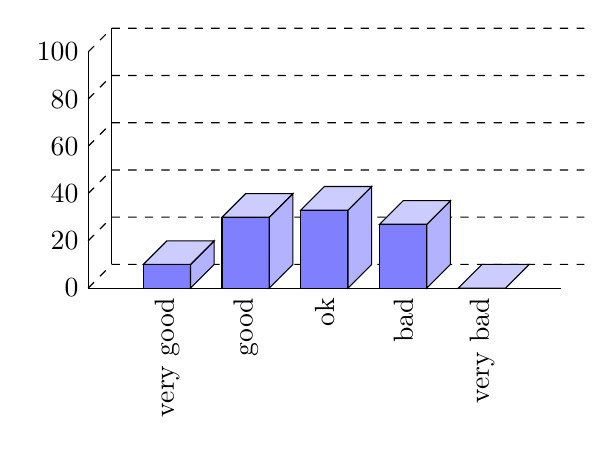
\begin{tikzpicture}[y=0.03cm,z=3mm]
  \foreach \y in {0,20,40,60,80,100}
    \draw[dashed] (0,\y,0) node[left] {\y} -- (0,\y,1)  -- (6,\y,1);

  \draw (0,0,0) -- (0,100,0)  (0,0,1) -- (0,100,1);
  \draw (0,0,0) -- (6,0,0);

  \foreach \x/\xtext/\height in {1/very good/10,2/good/30,3/ok/33,4/bad/27,5/very bad/0}
  {
    \draw (\x,0) node[rotate=90,anchor=east] {\xtext};

    \begin{scope}[xshift=\x cm]
      
    \filldraw[fill=blue!50] (-.3,0,0) rectangle (.3,\height,0);
    \filldraw[fill=blue!30] (.3,0,0) -- (.3,0,1) -- (.3,\height,1) -- (.3,\height,0) --cycle;
    \filldraw[fill=blue!20] (-.3,\height,0) -- (.3,\height,0) --
    (.3,\height,1) -- (-.3,\height,1) --cycle;
    \end{scope}
  }
\end{tikzpicture}
\bigskip

Both the table and the ``plot'' have about the same size. If your first
thought is ``the graphic looks nicer than the table,'' try to answer
the following questions based on the information in the table or in
the graphic: 
\begin{enumerate}
\item
  How many participants where there?
\item
  How many participants returned the feedback form?
\item
  What percentage of the participants returned the feedback form?
\item
  How many participants checked ``very good''?
\item
  What percentage out of all participants checked ``very good''?
\item
  Did more than a quarter of the participants check ``bad'' or ``very bad''?
\item
  What percentage of the participants that returned the form checked ``very good''?
\end{enumerate}

Sadly, the graphic does not allow us to answer \emph{a single one of these
  questions}. The table answers all of them directly, except for the last
one. In essence, the information density of the graphic is very
nearly zero. The table has a much higher information density; despite
the fact that it uses quite a lot of white space to present a few numbers.
Here is the list of things that went wrong with the 3D-bar diagram:
\begin{itemize}
\item
  The whole graphic is dominated by irritating background lines.
\item
  It is not clear what the numbers at the left mean; presumably
  percentages, but it might also be the absolute number of
  participants.
\item
  The labels at the bottom are rotated, making them hard to read.

  (In the real presentation that I saw, the text was rendered at a very 
  low resolution with about 10 by 6 pixels per letter with wrong
  kerning, making the rotated text almost impossible to read.)
\item
  The third dimension adds complexity to the graphic without adding
  information.
\item
  The three dimensional setup makes it much harder to gauge the height
  of the bars correctly. Consider the ``bad'' bar. It the number this
  bar stands for more than 20 or less? While the front of the bar is
  below the 20 line, the back of the bar (which counts) is above.
\item
  It is impossible to tell which  numbers are represented by the
  bars. Thus, the bars needlessly hide the information these bars are
  all about.
\item
  What do the bar heights add up to? Is it 100\% or 60\%?
\item
  Does the bar for ``very bad'' represent 0 or~1?
\item
  Why are the bars blue?
\end{itemize}

You might argue that in the example the exact numbers are not
important for the graphic. The important things is the ``message,''
which is that there are more ``very good'' and ``good'' ratings than
``bad'' and ``very bad.'' However, to convey this message either use a
sentence that says so or use a graphic that conveys this message more
clearly:  

\medskip
\par
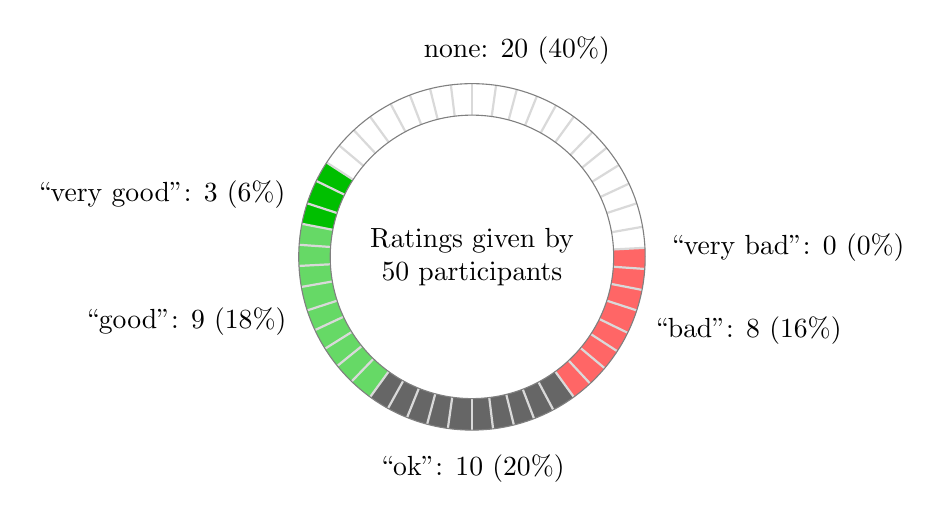
\begin{tikzpicture}
  \colorlet{good}{green!75!black}
  \colorlet{bad}{red}
  \colorlet{neutral}{black!60}
  \colorlet{none}{white}

  \node[align=center,text width=3cm]{Ratings given by 50~participants};

  \begin{scope}[line width=4mm,rotate=270]
    \draw[good]          (-123:2cm) arc (-123:-101:2cm);
    \draw[good!60!white] (-36:2cm) arc (-36:-101:2cm);
    \draw[neutral]       (-36:2cm) arc (-36:36:2cm);
    \draw[bad!60!white]  (36:2cm)  arc (36:93:2cm);

    \newcount\mycount
    \foreach \angle in {0,72,...,3599}
    {
      \mycount=\angle\relax
      \divide\mycount by 10\relax
      \draw[black!15,thick] (\the\mycount:18mm) -- (\the\mycount:22mm);
    }
    
    \draw (0:2.2cm) node[below] {``ok'': 10 (20\%)};
    \draw (165:2.2cm) node[above] {none: 20 (40\%)};
    \draw (-111:2.2cm) node[left] {``very good'': 3 (6\%)};
    \draw (-68:2.2cm) node[left] {``good'': 9 (18\%)};
    \draw (65:2.2cm) node[right] {``bad'': 8 (16\%)};
    \draw (93:2.2cm) node[right] {``very bad'': 0 (0\%)};
  \end{scope}  
  \draw[gray] (0,0) circle (2.2cm) circle (1.8cm);
\end{tikzpicture}

\bigskip
The above graphic has about the same information density as the table
(about the same size and the same numbers are shown). In addition, one
can directly ``see'' that there are more good or very good ratings
than bad ones. One can also ``see'' that the number of people who gave
no rating at all is not negligible, which is quite common for feedback
forms. 

Charts are not always a good idea. Let us look at an example
that I redrew from a pie chart in \emph{Die Zeit}, June 4th, 2005:

\bigskip
\par
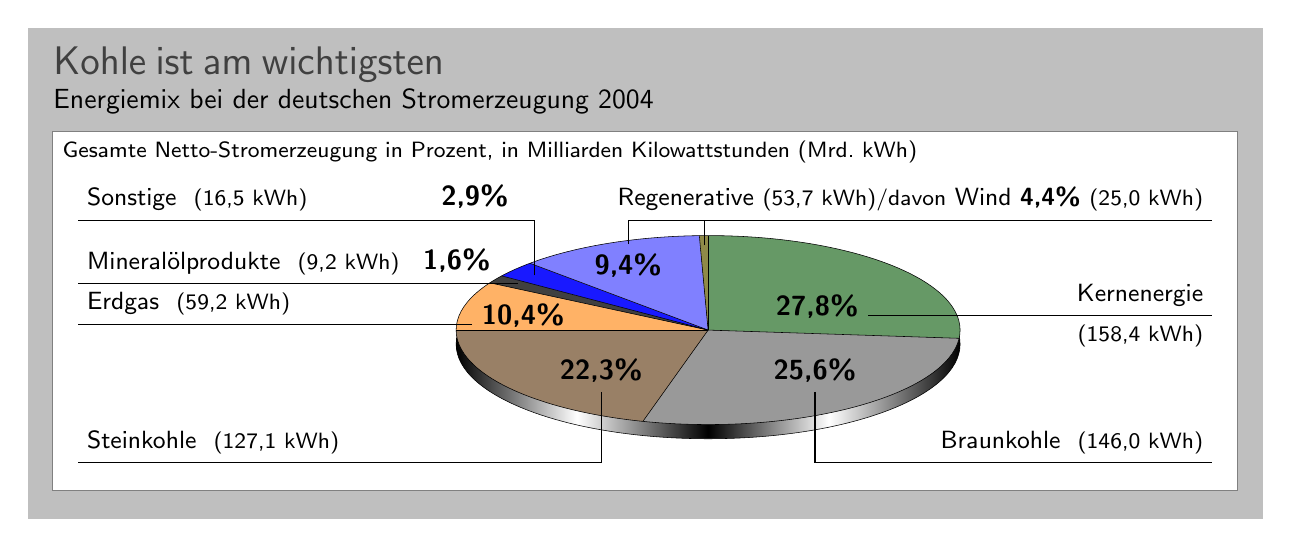
\begin{tikzpicture}
  \begin{scope}[xscale=3.2,yscale=1.2]

    \sffamily
    \coordinate (right border) at (2.0cm,-1.7cm);
    \coordinate (left border)  at (-2.5cm,2.1cm);

    \fill[black!25] ([xshift=-2mm,yshift=1.1cm]left border) rectangle ([xshift=2mm,yshift=-.3cm]right border);

    \node[below right,text width=10cm,inner sep=0pt] at ([yshift=.9cm,xshift=-1mm]left border)
    { {\color{black!75} \Large Kohle ist am wichtigsten}\\
      Energiemix bei der deutschen Stromerzeugung 2004};

    \filldraw[draw=gray,fill=white] ([xshift=-1mm]left border) node[below right,black]
      {\footnotesize Gesamte Netto-Stromerzeugung in Prozent, in
        Milliarden Kilowattstunden (Mrd.\ kWh)}
      rectangle ([xshift=1mm]right border);
    
    % The 3D stuff
    \pgfdeclarehorizontalshading{zeit}{100bp}
    {color(0pt)=(black);
      color(25bp)=(black);
      color(37bp)=(white);
      color(50bp)=(black);
      color(62bp)=(white);
      color(75bp)=(black);
      color(100bp)=(black)}

    \shadedraw[very thin,shading=zeit,yshift=-1.5mm] (0,0) circle (1cm);

    \fill[green!20!gray]   (0,0) -- (90:1cm) arc (90:-5:1cm);
    \fill[white!20!gray]   (0,0) -- (-5:1cm) arc (-5:-105:1cm);
    \fill[orange!20!gray]  (0,0) -- (-105:1cm) arc (-105:-180:1cm);
    \fill[orange!60!white] (0,0) -- (180:1cm) arc (180:150:1cm);
    \fill[black!75!white]  (0,0) -- (150:1cm) arc (150:145:1cm);
    \fill[blue!90!white]   (0,0) -- (145:1cm) arc (145:135:1cm);
    \fill[blue!50!white]   (0,0) -- (135:1cm) arc (135:92:1cm);
    \fill[yellow!50!black] (0,0) -- (92:1cm) arc (92:90:1cm);

    \begin{scope}[very thin]
      \draw (0,0) -- (90:1cm);
      \draw (0,0) -- (-5:1cm);
      \draw (0,0) -- (-105:1cm);
      \draw (0,0) -- (-180:1cm);
      \draw (0,0) -- (150:1cm);
      \draw (0,0) -- (145:1cm);
      \draw (0,0) -- (135:1cm);
      \draw (0,0) -- (92:1cm);
      
      \draw(0,0) circle (1cm);
    \end{scope}

    \node (Regenerative)   at (115:.75cm)  {\bfseries 9,4\%};
    \node (Kernenergie)    at (30:.5cm)   {\bfseries 27,8\%};
    \node (Braunkohle)     at (-45:.6cm)  {\bfseries 25,6\%};
    \node (Steinkohle)     at (-135:.6cm) {\bfseries 22,3\%};
    \node (Erdgas)         at (168:.75cm) {\bfseries 10,4\%};
    \coordinate (Mineral)  at (147:.9cm);
    \coordinate (Sonstige) at (140:.9cm);

    \small
    \draw (Regenerative.north) |- ([yshift=.25cm]Regenerative.north -| right border) coordinate (Regenerative label);
    \draw (91:.9cm) |- (Regenerative label);
    \node[above left] at (Regenerative label) {Regenerative\
      {\footnotesize (53,7 kWh)/davon} Wind \textbf{4,4\%}  \footnotesize (25,0 kWh)};

    \draw (Kernenergie.base east) -- (Kernenergie.base east -| right border) coordinate (Kernenergie label);
    \node[above left] at (Kernenergie label) {Kernenergie};
    \node[below left] at (Kernenergie label) {\footnotesize (158,4 kWh)};

    \draw (Braunkohle.south) |- ([yshift=-.75cm]Braunkohle.south -| right border) coordinate (Braunkohle label);
    \node[above left] at (Braunkohle label) {Braunkohle\ \ \footnotesize (146,0 kWh)};

    \draw (Steinkohle.south) |- ([yshift=-.75cm]Steinkohle.south -| left border) coordinate (Steinkohle label);
    \node[above right] at (Steinkohle label) {Steinkohle\ \ \footnotesize (127,1 kWh)};

    \draw (Erdgas.base west) -- (Erdgas.base west -| left border) coordinate (Erdgas label);
    \node[above right] at (Erdgas label) {Erdgas\ \ \footnotesize (59,2 kWh)};

    \draw (Mineral) -- (Mineral -| left border) coordinate (Mineral label);
    \node[above right] at (Mineral label) {Mineral\"olprodukte\ \
      \footnotesize (9,2 kWh) \  \ \normalsize\textbf{1,6\%}};

    \draw (Sonstige) |- (Regenerative label -| left border) coordinate (Sonstige label);
    \node[above right] at (Sonstige label) {Sonstige\ \
      \footnotesize (16,5 kWh) \hskip1.5cm\
      \normalsize\textbf{2,9\%}};
  \end{scope}    
\end{tikzpicture}

This graphic has been redrawn in \tikzname, but the original looks
almost exactly the same.

At first sight, the graphic looks  ``nice and informative,'' but there
are a lot of things that went wrong:

\begin{itemize}
\item
  The chart is three dimensional. However, the shadings add
  nothing ``information-wise,'' at best, they distract.
\item
  In a 3D-pie-chart the relative sizes are very strongly
  distorted. For example, the area taken up by the gray color of ``Braunkohle''
  is larger than the area taken up by the green color of
  ``Kernenergie'' \emph{despite the fact that the percentage of
    Braunkohle is less than the percentage of Kernenergie}.
\item
  The 3D-distortion gets worse for small areas. The area of
  ``Regenerative'' somewhat larger  than the area of ``Erdgas.''  
  The area of ``Wind'' is slightly smaller than the area of
  ``Mineral\"olprodukte'' \emph{although the percentage of Wind is
    nearly three times larger than the percentage of
    Mineral\"olprodukte.}

  In the last case, the different sizes are only partly due to
  distortion. The designer(s) of the original graphic have also made
  the ``Wind'' slice too small, even taking distortion into
  account. (Just compare the size of ``Wind'' to ``Regenerative'' in
  general.) 
\item
  According to its caption, this chart is supposed to inform us that
  coal was the most important energy source in Germany in
  2004. Ignoring the strong distortions caused by the superfluous and
  misleading 3D-setup, it takes quite a while for this message to get
  across. 

  Coal as an energy source is split up into two slices: one for
  ``Steinkohle'' and one for ``Braunkohle'' (two different kinds of
  coal). When you add them up, you see that the whole lower half of
  the pie chart is taken up by coal.

  The two areas for the different kinds of coal are not visually
  linked at all. Rather, two different colors are used, the labels are
  on different sides of the graphic. By comparison, ``Regenerative''
  and ``Wind'' are very closely linked.
\item
  The color coding of the graphic follows no logical pattern at
  all. Why is nuclear energy green? Regenerative energy is light blue,
  ``other sources'' are blue. It seems more like a joke that the area
  for ``Braunkohle'' (which literally translates to ``brown coal'') is
  stone gray, while the area for ``Steinkohle'' (which literally
  translates to ``stone coal'') is brown.
\item
  The area with the lightest color is used for ``Erdgas.'' This area
  stands out most because of the brighter color. However, for this
  chart ``Erdgas'' is not really important at all.
\end{itemize}
Edward Tufte calls graphics like the above ``chart junk.'' (I am happy
to announce, however, that \emph{Die Zeit} has stopped using 3D pie
charts and their information graphics have got somewhat better.)

Here are a few recommendations that may help you avoid producing chart junk:
\begin{itemize}
\item
  Do not use 3D pie charts. They are \emph{evil}.
\item
  Consider using a table instead of a pie chart.
\item
  Due not apply colors randomly; use them to direct the readers's 
  focus and to group things.
\item
  Do not use background patterns, like a crosshatch or diagonal
  lines, instead of colors. They distract. Background patterns in
  information graphics are \emph{evil}.
\end{itemize}



\subsection{Attention and Distraction}

Pick up your favorite fiction novel and have a look at a typical
page. You will notice that the page is very uniform. Nothing is there
to distract the reader while reading; no large headlines, no bold
text, no large white areas. Indeed, even when the author does wish to
emphasize something, this is done using italic letters. Such letters
blend nicely with the main text---at a distance you will not be able to
tell whether a page contains italic letters, but you would notice a
single bold word immediately. The reason novels are typeset this way
is the following paradigm: Avoid distractions.

Good typography (like good organization) is something you do
\emph{not} notice. The job of typography is to make reading the text,
that is, ``absorbing'' its information content, as effortless as
possible. For a novel, readers absorb the content by reading the text
line-by-line, as if they were listening to someone telling the
story. In this situation anything on the page that distracts the eye
from  going quickly and evenly from line to line will make the text
harder to read.

Now, pick up your favorite weekly magazine or newspaper and have a
look at a typical 
page. You will notice that there is quite a lot ``going on'' on the
page. Fonts are used at different sizes and in different arrangements,
the text is organized in narrow columns, typically interleaved with
pictures. The reason magazines are typeset in this way is another
paradigm: Steer attention.

Readers will not read a magazine like a novel. Instead of reading a
magazine line-by-line, we use headlines and short abstracts to check
whether we want to read a certain article or not. The job of
typography is to steer our attention to these abstracts and headlines,
first. Once we have decided that we want to read an article, however,
we no longer tolerate distractions, which is why the main text of
articles is typeset exactly the same way as a novel.

The two principles ``avoid distractions'' and ``steer attention'' also
apply to graphics. When you design a graphic, you should eliminate
everything that will ``distract the eye.'' At the same time, you
should try to actively help the reader ``through the graphic'' by
using fonts/colors/line widths to highlight different parts.

Here is a non-exhaustive list of things that can distract readers:
\begin{itemize}
\item
  Strong contrasts will always be registered first by the eye. For
  example, consider the following two grids:

  \medskip\par
  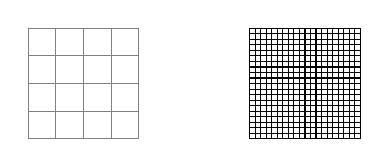
\begin{tikzpicture}[x=40pt,y=40pt]
    \draw[step=10pt,gray] (0,0) grid +(1,1);
    \draw[step=2pt]      (2,0) grid +(1,1);
  \end{tikzpicture}

  \medskip
  Even though the left grid comes first in English reading order,
  the right one is much more likely to be seen first: The
  white-to-black contrast is higher than the gray-to-white
  contrast. In addition, there are more ``places'' adding to the
  overall contrast in the right grid.

  Things like grids and, more generally, help lines usually should not
  grab the attention of the readers and, hence, should be typeset with
  a low contrast to the background. Also, a loosely-spaced grid is
  less distracting than a very closely-spaced grid.
\item
  Dashed lines create many points at which there is black-to-white
  contrast. Dashed or dotted lines can be very distracting and, hence,
  should be avoided in general.

  Do not use different dashing patterns to differentiate curves in
  plots. You loose data points this way and the eye is not
  particularly good at ``grouping things according to a dashing
  pattern.'' The eye is \emph{much} better at grouping things
  according to colors.
\item
  Background patterns filling an area using  diagonal lines or
  horizontal and vertical lines or just dots are almost always
  distracting and, usually, serve no real purpose.
\item
  Background images and shadings distract and only seldom add
  anything of importance to a graphic.
\item
  Cute little cliparts can easily draw attention away from the
  data.
\end{itemize}

